\documentclass[11pt, a4paper, english]{NTNUoving}
\usepackage[utf8]{inputenc}
\usepackage[T1]{fontenc}
\usepackage{amsfonts}

\ovingnr{}    % Nummer på innlevering
\semester{Compulsory exercise 1}
\fag{TMA4267 - Linear statistical models}
\institutt{Institutt for matematiske fag}


\begin{document}

%\begin{punkt}
%\input{oppg_1a}
%\end{punkt}

\section*{Bivariate normal distribution}
\textbf{a)}
Use $\textbf{X}$ and $\textbf{Y}$ as given in the problem set.

%\textbf{Y} =  \begin{pmatrix}
%1/ \sqrt{2} & - 1/ \sqrt{2} \\
%1/ \sqrt{2}  & 1/ \sqrt{2} 
%\end{pmatrix}  \textbf{X}

Define C =  \begin{pmatrix}
1/ \sqrt{2} & - 1/ \sqrt{2} \\
1/ \sqrt{2}  & 1/ \sqrt{2} 
\end{pmatrix}, so $\textbf{Y} = C\textbf{X}$

The mean vector of Y:

$$E[\textbf{Y}] = E[C \textbf{X}] = C E[\textbf{X}] = \begin{pmatrix}
1/ \sqrt{2} & - 1/ \sqrt{2} \\
1/ \sqrt{2}  & 1/ \sqrt{2} 
\end{pmatrix} \begin{pmatrix}
0 \\
2  
\end{pmatrix} = \begin{pmatrix}
- \sqrt{2}\\
\sqrt{2}  
\end{pmatrix} .$$


The covariance matrix of Y : 

$$\text{Cov}[\textbf{Y}] = \text{Cov}(C\textbf{X}) = C \cdot \text{Cov}(\textbf{X}) \cdot C^T $$ $$= \begin{pmatrix}
1/ \sqrt{2} & - 1/ \sqrt{2} \\
1/ \sqrt{2}  & 1/ \sqrt{2} 
\end{pmatrix} \begin{pmatrix}
3 & 1 \\
1  & 3
\end{pmatrix} \begin{pmatrix}
1/ \sqrt{2} &  1/ \sqrt{2} \\
- 1/ \sqrt{2}  & 1/ \sqrt{2} 
\end{pmatrix} = \begin{pmatrix}
2 & 0\\
0  & 4 
\end{pmatrix} $$


Since Y is a linear combination of X, which is bivariate normal distributed, the distribution of \textbf{Y} is bivariate normal distributed with mean $(-\sqrt{2}, \sqrt{2})^T$, and covariance matrix $\begin{pmatrix}
2 & 0\\
0  & 4 
\end{pmatrix} $

$$\textbf{Y } \mathtt{\sim} \text{ N}\left(\begin{pmatrix}
-\sqrt{2} \\
\sqrt{2}
\end{pmatrix} , \begin{pmatrix}
2 & 0\\
0  & 4 
\end{pmatrix}\right) $$

$Y_1$ and $Y_2$ are independent variables since $\text{Cov}(Y_1, Y_2) = 0$ according to the covariance matrix of $Y$. 

%if one choose $A$ and $B$ such that $AY = Y_1$ and $BY = Y_2$ then $A \Sigma B^T = 0$



\textbf{b)}
Let $\text{E}_b = \{ x \in \mathbb{R}^2 | (\mathbf{x} - \mathbf{\mu})^T \Sigma^{-1}(\mathbf{x} - \mathbf{\mu}) = b \}$ be the ellipsoid shown in the figure, which is centered in $\mathbf{\mu} = \text{E}[X] = [0 \quad 2]^T$. Applying Theorem 2.7 in Härdle and Simar, we can determine that the principal axes of $\text{E}_b$ will be in the direction of the eigenvectors of $\Sigma^{-1}$ and that their half-lengths will be given by $\sqrt{\frac{b}{\lambda_i}}$, $i =1,2$ where $\lambda_i$ are the eigenvalues of $\Sigma^{-1}$.

We know that $\Sigma$ and $\Sigma^{-1}$ share the same eigenvectors and that the eigenvalues of $\Sigma^{-1}$ are  $\Tilde{\lambda_i}= \frac{1}{{\lambda_i}}$ where $\lambda_i$ are the eigenvalues of $\Sigma$. 
Thus, the principal axes of $\text{E}_b$ lie along $[\: 1 \;  1\: ]^T$ and $[\: 1 \ -1\:]^T$, and the lengths of the half-lengths are $d_1 = \sqrt{2b} \approx 3.03$ and $d_2 =  \sqrt{4b} \approx 4.29$.
%%%jeg lurer på om det burde vært b^2 i ligningen for ellipsen? og vi må lage figur her og legge inn, derfor jeg har brukt navn d1 og d2


$(\mathbf{x}- \mathbf{\mu})^T\Sigma^{-1} (\mathbf{x}- \mathbf{\mu})$ defines a distance from the centre $\mathbf{\mu}$, so that for all points $\mathbf{x} \in \text{E}_b$, $\mathbf{x} \leq b$. 
Using the Mahalanobis transformation, we recognize that 
\begin{equation*}
    (\mathbf{x}- \mathbf{\mu})^T\Sigma^{-1} (\mathbf{x}- \mathbf{\mu})
    = (\mathbf{x}- \mathbf{\mu})^T(\Sigma^{-1/2})^T\Sigma^{-1/2}(\mathbf{x}- \mathbf{\mu}) = Z^TZ = \sum_{i=1}^p z_i^2
\end{equation*}

where $Z \sim N(\mathbf{0}, \sigma^2 I)$ so that $z_i \sim N(0,\sigma^2)$ and $z_i^2 \sim \mathcal{X}_1^2$. As a sum of p $\mathcal{X}_1^2$ variables, $(\mathbf{x}- \mathbf{\mu})^T\Sigma^{-1} (\mathbf{x}- \mathbf{\mu})$ is thus $\mathcal{X}_p^2$ distributed with $\text{p}=2$. %%må noe av dette vises? idk

Accordingly, the probability that $\mathbf{X}$ falls within the given ellipse is given by the chi-squared distribution, $\text{P}(\mathbf{X} \leq 4.6) = 0.9$.


\begin{figure}
    \centering
    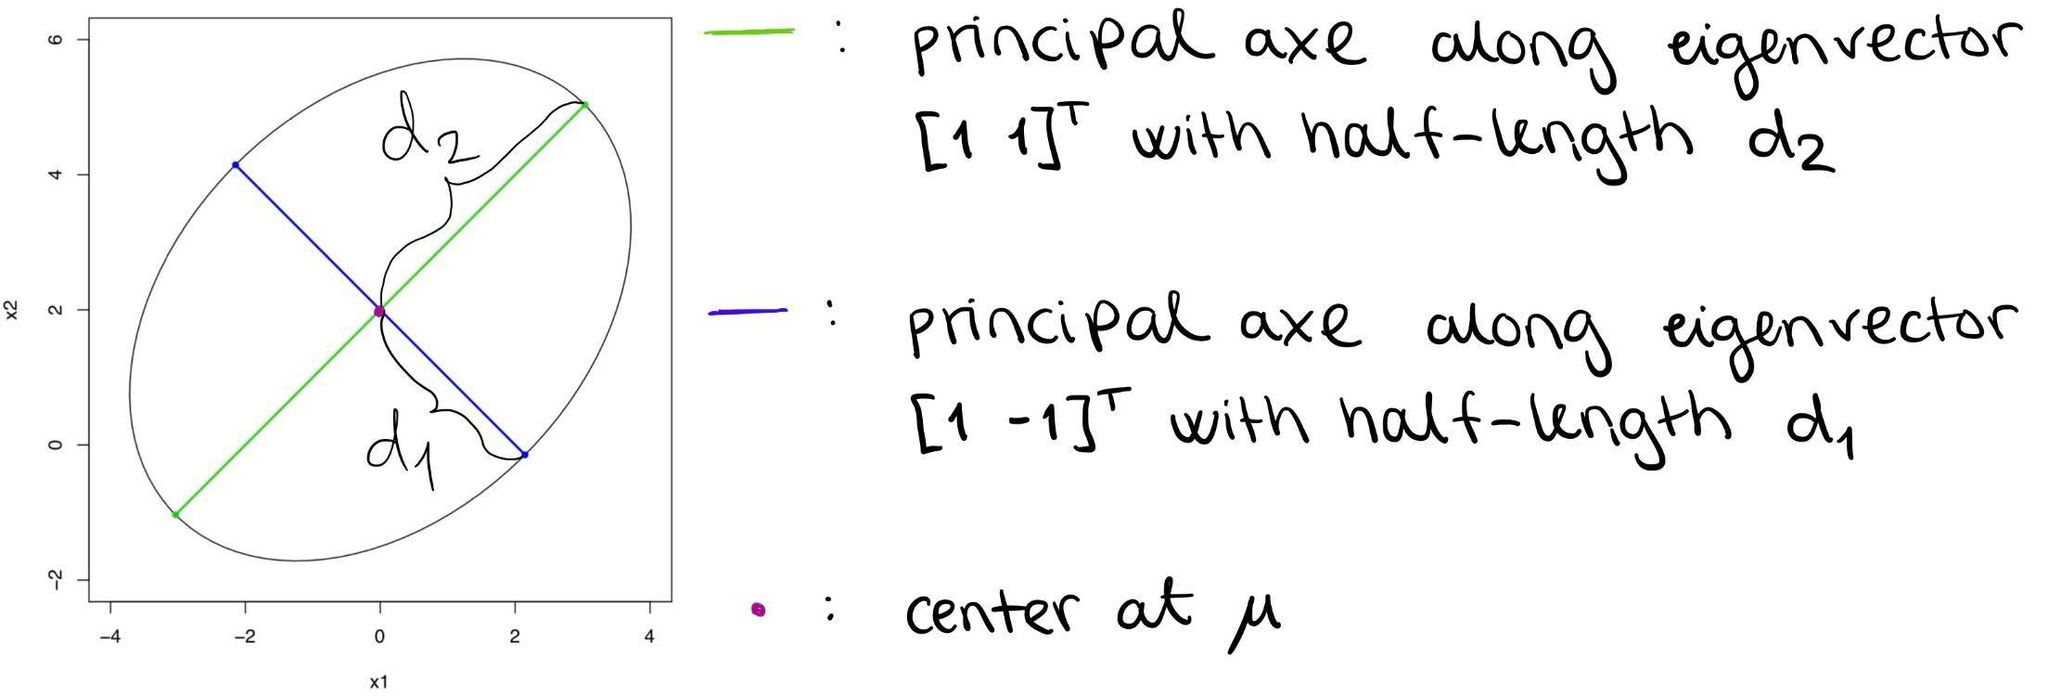
\includegraphics[width=1\textwidth]{figur1.jpg}
    \caption{}
    \label{figure}
\end{figure}


\section*{Distributional results for $\bar{X}$ and $S^2$ for a univariate normal sample}
\textbf{a)}
First, we want to show that the mean value of X given as $\bar X = \frac{1}{n} \sum_{i=1}^{n} X_i$, can be written as $\bar X = \frac{1}{n} \textbf{1}^T \textbf{X}$. 
$$
\bar X = \frac{1}{n} \sum_{i=1}^{n} X_i = \frac{1}{n} (X_1 + X_2 + ... + X_n) = \frac{1}{n} [1, 1, ..., 1]^T [X_1, X_2, ..., X_n]= \frac{1}{n} \textbf{1}^T \textbf{X}
$$

Secondly, we want to show that the estimator of the variance $S^2 = \frac{1}{n-1}  \sum_{i=1}^{n} (X_i - \bar X)^2$ can be written in terms of the centering matrix C as  $S^2 = \frac{1}{n-1} \textbf{X}^T C \textbf{X}.$
$$
S^2 = \frac{1}{n-1}  \sum_{i=1}^{n} (X_i - \bar X)^2 = \frac{1}{n-1} (C\textbf{X})^T (C\textbf{X}) = \frac{1}{n-1} \textbf{X}^T C^T C \textbf{X} =  \frac{1}{n-1} \textbf{X}^T C \textbf{X}
$$

Here, $\sum_{i=1}^{n} (X_i - \bar X)^2 = (C\textbf{X})^T (C\textbf{X})$ since ...

and the final equality is due to the fact the the centering matrix is symmetric and idempotent, so that $C^T C = CC = C^2 = C$.  



\textbf{b)}
First we will show that $\frac{1}{n}\textbf{1}^T C = \textbf{0}^T$. 

$$\frac{1}{n}\textbf{1}^T C = \frac{1}{n} \textbf{1}^T \left(I - \frac{1}{n} \textbf{1}\textbf{1}^T\right) = \frac{1}{n} \textbf{1}^T - \frac{1}{n^2} \textbf{1}^T \textbf{1}\textbf{1}^T = \frac{1}{n} \textbf{1}^T - \frac{1}{n} \textbf{1}^T = \textbf{0}^T$$

where we have used that $\textbf{1}^T \textbf{1} = n$.

If we define $A = \frac{1}{n} \textbf{1}^T$, then we can say that $A \textbf{X}$ and $C \textbf{X}$ are independent if $A \Sigma C^T = 0$.

Using that both the centering and the identity matrix are symmetric idempotent one get
$$ 
A \Sigma C^T = A \Sigma C =  \frac{1}{n} \textbf{1}^T \sigma^2 I (I - \frac{1}{n} \textbf{1}\textbf{1}^T) = \frac{ \sigma^2}{n} \textbf{1}^T I^2 - \frac{\sigma^2}{n^2}  \textbf{1}^T  \textbf{1}\textbf{1}^T I =  \frac{ \sigma^2}{n} \textbf{1}^T I - \frac{ \sigma^2}{n} \textbf{1}^T I = 0.
$$
So, $\frac{1}{n} \textbf{1}^T X$ and $C\textbf{X}$ are independent, which can also been seen from what we showed above, namely that $\frac{1}{n} \textbf{1}^T C = \textbf{0}^T $, meaning that (the product of) each component is orthogonal/uncorrelated/independent ???????????

Furthermore, this result can be used to conclude that $\bar X$ and $S^2$ are independent, since 




\textbf{c)}
Here we are going to derive the distribution of $\frac{(n-1)S^2}{\sigma^2}$, where $S^2 = \frac{1}{n-1}\boldsymbol{X}^TC\boldsymbol{X}$, $C$ is the centring matrix and $\boldsymbol{X} \sim N(\mu\boldsymbol{1}, \sigma^2I)$. We want to use that if $R$ is a symmetric and idempotent matrix with rank $r$, and $\boldsymbol{Y} \sim N(\boldsymbol{0}, I)$, then $\boldsymbol{Y}^TR\boldsymbol{Y} \sim \chi_r^2$, as stated in the hint in the problem. We cannot use this directly since $\boldsymbol{X}$ is not standard normal distributed. Hence, we start by using the Mahalanobis transformation,
\begin{equation}
    \label{mahalonobis}
    \boldsymbol{Z} = \Sigma^{-1/2}(\boldsymbol{X} -\boldsymbol{\mu}) \implies \boldsymbol{X} = \Sigma^{1/2}\boldsymbol{Z} +\boldsymbol{\mu}.
\end{equation}

By substitute $\boldsymbol{X}$ in $S^2 = \frac{1}{n-1}\boldsymbol{X}^TC\boldsymbol{X}$ by \eqref{mahalonobis}, with $\Sigma^{1/2} = \sigma I$ and $\boldsymbol{\mu} = \mu \boldsymbol{1}$, we get

\begin{align*}
    S^2 &= \frac{1}{n-1}\left(\sigma I\boldsymbol{Z}+\mu\boldsymbol{1}\right)^TC\left(\sigma I\boldsymbol{Z}+\mu\boldsymbol{1}\right)\\
    &= \frac{1}{n-1}\left(C\left(\sigma I\boldsymbol{Z}+\mu\boldsymbol{1}\right)\right)^TC\left(\sigma I\boldsymbol{Z}+\mu\boldsymbol{1}\right)\\
    &= \frac{1}{n-1}\left(\left(I-\frac{1}{n}\boldsymbol{1}\boldsymbol{1}^T\right)\left(\sigma I\boldsymbol{Z}+\mu\boldsymbol{1}\right)\right)^T\left(I-\frac{1}{n}\boldsymbol{1}\boldsymbol{1}^T\right)\left(\sigma I\boldsymbol{Z}+\mu\boldsymbol{1}\right) \\
    &= \frac{1}{n-1}\left(\sigma\boldsymbol{Z}+\mu\boldsymbol{1}-\frac{\sigma}{n}\boldsymbol{1}\boldsymbol{1}^T\boldsymbol{Z}-\frac{\mu}{n}\boldsymbol{1}\boldsymbol{1}^T\boldsymbol{1}\right)^T\left(\sigma\boldsymbol{Z}+\mu\boldsymbol{1}-\frac{\sigma}{n}\boldsymbol{1}\boldsymbol{1}^T\boldsymbol{Z}-\frac{\mu}{n}\boldsymbol{1}\boldsymbol{1}^T\boldsymbol{1}\right) \\
    &= \frac{1}{n-1}\left(\sigma\boldsymbol{Z}-\frac{\sigma}{n}\boldsymbol{1}\boldsymbol{1}^T\boldsymbol{Z}\right)^T\left(\sigma\boldsymbol{Z}-\frac{\sigma}{n}\boldsymbol{1}\boldsymbol{1}^T\boldsymbol{Z}\right) \\
    &= \frac{\sigma^2}{n-1}\left(\left(I-\frac{1}{n}\boldsymbol{1}\boldsymbol{1}^T\right)\boldsymbol{Z}\right)^T\left(\left(I-\frac{1}{n}\boldsymbol{1}\boldsymbol{1}^T\right)\boldsymbol{Z}\right) \\
    &= \frac{\sigma^2}{n-1}\boldsymbol{Z}^TC\boldsymbol{Z},
\end{align*}

where we have used that $C$ is idempotent and symmetric and that $\boldsymbol{1}^T\boldsymbol{1} = n$. This implies that 
\begin{equation*}
    \frac{(n-1)S^2}{\sigma^2} = \boldsymbol{Z}^TC\boldsymbol{Z},
\end{equation*}

and since $\boldsymbol{Z} \sim N(\boldsymbol{0}, I)$ and $\text{rank}(C) = \text{tr}(C) = n - 1$ is 

\begin{equation*}
    \frac{(n-1)S^2}{\sigma^2} \sim \chi_{n-1}^2.
\end{equation*}



\end{document}

